% =====================================================================
% Section V (Experiments) of the 1015 draft, input from Papers/1015/main.tex.
% Defines: sec:experiments, subsec:exp-setup, subsec:exp-comparison, subsec:exp-ablation,
%   subsec:exp-mechanism, tab:exp-scales, tab:exp-methods, tab:exp-main, tab:exp-ablation,
%   fig:exp-generalization, fig:exp-capacity, fig:exp-memory, fig:exp-depth.
% Uses: subsec:pf-scenario, subsec:pf-decpomdp, subsec:pf-attacker, eq:fw-reward (Section III),
%   sec:method, subsec:method-loop, subsec:method-memory, subsec:method-training, prop:selection,
%   prop:prefix (Section IV).
% Packages already loaded by main.tex: booktabs, multirow, graphicx.
% New references: listed in sections/sec_5_6/references_sec5_6.bib and merged into Papers/1015/references.bib.
% Figures: figures/exp_*.pdf, rendered by figures/src/figures.py from Open-SCORE/outputs/main.
%   Table rows: python figures/src/figdata.py --tables.
% Vehicle model: kept generic. Dynamics and engagement constants appear only in Section III.
% =====================================================================

\section{Experiments}
\label{sec:experiments}

This section answers three questions. Does a policy trained once on small engagements protect targets better than existing methods when it is deployed at larger scales? Which designs of LEAF produce this generalization? Why do these designs work? Section~\ref{subsec:exp-setup} describes the setup, and Sections~\ref{subsec:exp-comparison} to~\ref{subsec:exp-mechanism} answer the three questions in turn.

\begin{table}[!t]
\centering
\footnotesize
\setlength{\tabcolsep}{4pt}
\caption{Scale protocol. Configurations are written $(N,K)$ with $N=N_R=N_B$.}
\label{tab:exp-scales}
\begin{tabular}{@{}llc@{}}
\toprule
Set & Configurations $(N,K)$ & Count\\
\midrule
Training & $N\in\{4,6,8,10\}$, $K\in\{1,2,3\}$, drawn per episode & --\\
ID & (4,2), (6,2), (8,2), (10,3) & 4\\
$K$-OOD & (10,4), (10,6), (10,9), (10,12) & 4\\
$N$-OOD & (15,2), (20,2), (25,2), (30,2), (40,2), (50,2) & 6\\
\multirow{2}{*}{Joint-OOD} & (15,4), (15,6), (20,4), (20,6), & \multirow{2}{*}{8}\\
 & (30,4), (30,6), (30,9), (30,12) & \\
Extra & (5,2), (10,2) & 2\\
\bottomrule
\end{tabular}
\vspace{2pt}

\parbox{\columnwidth}{\footnotesize Every evaluation configuration uses the same 300 initial scenes for all methods. The two extra configurations enter only the scale sweeps of Fig.~\ref{fig:exp-generalization} and the averages over all 24 configurations.}
\end{table}

\begin{table}[!t]
\centering
\footnotesize
\setlength{\tabcolsep}{3pt}
\caption{Compared methods. Parameters count the networks used at deployment.}
\label{tab:exp-methods}
\begin{tabular}{@{}l p{0.53\columnwidth} c r@{}}
\toprule
Method & Coordination mechanism & Target & Params\\
\midrule
QMIX & Self-query entity attention, monotonic entity mixer & DQ & 102k\\
REFIL & QMIX with randomly grouped imagined entity views & DQ & 102k\\
DCG & Utilities and pairwise payoffs on a complete coordination graph & DQ & 112k\\
ALMA & Learned target allocation and allocation-conditioned actor & DQ & 283k\\
TransfQMix & Transformer actor and mixer with a memory token & TD($\lambda$) & 51k\\
SPECTra & Typed set projections, self-query read, set mixer & TD($\lambda$) & 47k\\
Rule & Integer assignment with predicted interception at every step & -- & --\\
LEAF & Looped threat context on the REFIL host & DQ & 176k\\
\bottomrule
\end{tabular}
\vspace{2pt}

\parbox{\columnwidth}{\footnotesize DQ denotes one-step double Q-learning with RMSprop, and TD($\lambda$) denotes $\lambda$-returns with Adam, as in the original implementations. All learned methods carry recurrent memory.}
\end{table}

\begin{table*}[!t]
\centering
\footnotesize
\setlength{\tabcolsep}{3.4pt}
\caption{Zero-shot results on the four test groups. Damage $D$ gives the mean and SD over three training seeds, and $P$ and CVaR give seed means. The best value in each column is in bold and the second best is underlined.}
\label{tab:exp-main}
\begin{tabular}{@{}l cccc c cccc c cccc@{}}
\toprule
& \multicolumn{4}{c}{Damage $D\downarrow$} && \multicolumn{4}{c}{Damage incidence $P$ (\%)\,$\downarrow$} && \multicolumn{4}{c}{Tail damage CVaR\,$\downarrow$}\\
\cmidrule{2-5}\cmidrule{7-10}\cmidrule{12-15}
Method & ID & $K$-OOD & $N$-OOD & Joint && ID & $K$-OOD & $N$-OOD & Joint && ID & $K$-OOD & $N$-OOD & Joint\\
\midrule
QMIX & 2.32$\pm$1.43 & 5.01$\pm$2.50 & 5.14$\pm$3.11 & 7.42$\pm$3.97 && 82.1 & 92.9 & 92.0 & 94.4 && 5.18 & 10.94 & 11.57 & 15.98\\
REFIL & \underline{0.72}$\pm$0.05 & \underline{1.80}$\pm$0.30 & 2.21$\pm$0.28 & 3.31$\pm$0.30 && \underline{44.4} & \underline{60.4} & \underline{67.0} & \underline{73.2} && \underline{2.79} & \underline{6.18} & 7.81 & 10.66\\
DCG & 2.03$\pm$0.44 & 5.84$\pm$1.92 & 5.02$\pm$2.66 & 8.09$\pm$3.91 && 85.2 & 96.4 & 94.8 & 97.9 && 4.99 & 12.07 & 11.77 & 17.32\\
ALMA & 1.33$\pm$0.19 & 3.02$\pm$0.34 & 3.61$\pm$0.74 & 5.37$\pm$1.04 && 67.8 & 83.0 & 90.3 & 92.6 && 3.86 & 7.78 & 9.10 & 12.97\\
TransfQMix & 1.53$\pm$0.28 & 3.95$\pm$0.50 & 4.02$\pm$0.97 & 6.63$\pm$1.20 && 68.5 & 88.1 & 89.5 & 93.9 && 4.39 & 9.63 & 10.84 & 15.87\\
SPECTra & 2.48$\pm$0.21 & 6.74$\pm$0.53 & 5.05$\pm$0.59 & 9.84$\pm$0.49 && 90.9 & 98.9 & 95.6 & 99.3 && 5.71 & 13.30 & 12.09 & 19.49\\
Rule$^\dagger$ & 1.46$\pm$0.72 & 3.21$\pm$1.13 & \underline{1.54}$\pm$0.88 & \underline{3.06}$\pm$0.98 && 80.2 & 92.6 & 75.1 & 88.9 && 3.77 & 7.15 & \underline{4.67} & \underline{7.70}\\
LEAF & \textbf{0.41}$\pm$0.10 & \textbf{1.00}$\pm$0.23 & \textbf{0.57}$\pm$0.23 & \textbf{1.10}$\pm$0.10 && \textbf{27.6} & \textbf{41.4} & \textbf{31.4} & \textbf{39.1} && \textbf{2.10} & \textbf{4.14} & \textbf{3.10} & \textbf{5.41}\\
\midrule
LEAF vs.\ best & $-$43\% & $-$45\% & $-$63\% & $-$64\% && $-$38\% & $-$31\% & $-$53\% & $-$47\% && $-$25\% & $-$33\% & $-$34\% & $-$30\%\\
\bottomrule
\end{tabular}
\vspace{2pt}

\parbox{\textwidth}{\footnotesize $^\dagger$Rule has no training seeds, and its SD is taken over scenes. Joint denotes Joint-OOD. CVaR is the mean damage of the worst 30 of the 300 episodes in each configuration. The last row compares LEAF with the best other method in each column.}
\end{table*}

\begin{figure*}[!t]
\centering
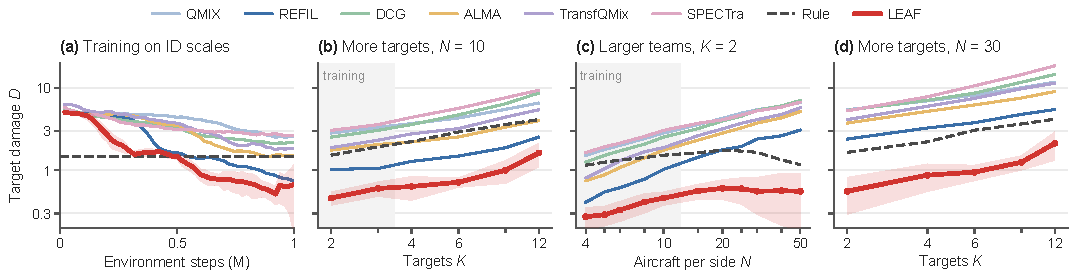
\includegraphics[width=\textwidth]{figures/exp_generalization.pdf}
\caption{Learning and zero-shot scale generalization. (a) Damage on the ID validation scenes during training, smoothed over five consecutive validation points. The dashed line marks the ID damage of Rule. (b)--(d) Damage of the frozen final policies as the number of targets grows at $N=10$, as the team grows at $K=2$, and as the number of targets grows at $N=30$, beyond the training team size. Gray shading marks the training range. Each point averages 300 common scenes and three training seeds, and the red band shows one SD of LEAF over the seeds. Table~\ref{tab:exp-main} lists the SDs of all methods.}
\label{fig:exp-generalization}
\end{figure*}

\subsection{Experimental Setup}
\label{subsec:exp-setup}

\emph{Task and scale protocol.} All experiments use the SkyHAD Damage task of Section~\ref{subsec:pf-scenario}. $N$ defenders protect $K$ stationary targets against $N$ attackers that follow the rule of Section~\ref{subsec:pf-attacker}, and an episode ends when all attackers are destroyed or after 100 decisions. During training, every episode draws its own configuration with $N\in\{4,6,8,10\}$ and $K\in\{1,2,3\}$. The frozen policies are then deployed on the configurations of Table~\ref{tab:exp-scales}. These form an in-distribution (ID) group and three out-of-distribution (OOD) groups that enlarge the number of targets, the team size, or both, which we call $K$-OOD, $N$-OOD, and Joint-OOD. Two extra configurations inside the training range complete the scale sweeps. The largest deployments have five times as many aircraft per side or four times as many targets as the largest training configuration. Training adds a potential-based shaping term to the team reward \eqref{eq:fw-reward}, which leaves the optimal policy unchanged~\cite{ng1999shaping}. All reported results use the unshaped episode damage.

\emph{Baselines.} We compare LEAF with six learned baselines and a rule-based controller, summarized in Table~\ref{tab:exp-methods}. Each represents one approach to scalable cooperative defense. QMIX~\cite{rashid2018qmix} and REFIL~\cite{iqbal2021refil} factorize the team value, and each defender reads the raw entities once with a query formed from its own state. We use QMIX in its entity-attention form with the entity mixer of REFIL. REFIL is the host of LEAF and thus its closest comparison. DCG~\cite{boehmer2020dcg} models pairwise coordination at the level of actions. ALMA~\cite{iqbal2022alma} first allocates defenders to targets and then maneuvers, the decomposition common in defense automation. TransfQMix~\cite{transfqmix2023} and SPECTra~\cite{park2026spectra} were designed for scalability. TransfQMix relates the entities and a memory token over several Transformer layers, and SPECTra encodes typed entity sets before a self-query read. Rule represents optimization-based engineering practice. At every step, it selects the attackers closest to the defenders, at most as many as there are living defenders, and solves a 0--1 integer program. The program assigns every defender to one selected attacker and covers every selected attacker while minimizing the total distance between the defenders and the attacker positions predicted one step ahead at constant velocity. Each defender then takes the acceleration intent closest to the velocity that intercepts its attacker. Like the attacker rule of Section~\ref{subsec:pf-attacker}, Rule separates assignment from steering.

\emph{Common adaptation.} All learned methods use the entity observation of Section~\ref{subsec:pf-decpomdp} with the same features and masks, the same intent set, the same attackers, the same training distribution, and $10^6$ environment steps per training run. Each method keeps its architecture and learning rule, and we replace only its input interface, action head, and masks. Each method also handles variable scale with its own mechanism. QMIX, REFIL, ALMA, and LEAF use the attention-based entity mixer of REFIL, SPECTra uses its set hypernetwork mixer, and TransfQMix uses its Transformer mixer. DCG builds a complete coordination graph over the deployed team, and ALMA treats each target as a subtask.

\emph{Training.} Every method is trained with three seeds. Eight parallel environments collect data, and each collection round is followed by eight updates on minibatches of 32 episodes from a replay buffer of 5000 episodes. All methods use a discount of 0.99, gradient clipping at 10, hard target updates every 200 episodes, and $\epsilon$-greedy exploration annealed from 1.0 to 0.05 over $10^5$ steps, or $5\times10^4$ steps for DCG. LEAF, QMIX, REFIL, DCG, and ALMA use RMSprop with a learning rate of $5\times10^{-4}$ and one-step double Q-learning targets~\cite{vanhasselt2016double}. SPECTra and TransfQMix keep Adam with a learning rate of $10^{-3}$ and $\lambda$-returns with $\lambda=0.6$ from their implementations. LEAF uses the architecture of Section~\ref{subsec:method-training}, samples $L$ uniformly from one to four during training, and executes $L_{\mathrm{exec}}=4$ rounds unless stated otherwise. Every $2\times10^4$ steps, each run is evaluated on the four ID configurations with 25 episodes each from a separate scene pool. These 50 validation points produce the learning curves and play no role in model selection.

\emph{Evaluation and metrics.} Evaluation is zero-shot. We take the final weights at the end of the budget, freeze them, select intents greedily, and apply no fine-tuning. Every model runs the same 300 initial scenes in every configuration. The attackers react to the defenders, so one initial scene can unfold differently under different policies, as closed-loop evaluation requires. The primary metric is the episode damage $D$ of Section~\ref{subsec:pf-decpomdp}, summed over all targets without capping. Two further metrics describe the quality of protection. The damage incidence $P$ is the fraction of episodes in which at least one target is damaged. The conditional value at risk (CVaR) is the mean damage of the worst 10\% of episodes in a configuration and measures tail risk. The mechanism analyses also report the fraction $I$ of attackers that are intercepted and the fraction $C$ of defenders lost to friendly collisions. For every trained model, we average over the scenes of a configuration and then over the configurations of a group with equal weight. We report the mean and the sample standard deviation (SD) over the three training seeds. Rule has no training seed, and its SD is taken over scenes. With three seeds per method, we state comparisons at the level of individual seeds, which readers can check directly~\cite{agarwal2021rliable}.

\begin{table*}[!t]
\centering
\footnotesize
\setlength{\tabcolsep}{2.5pt}
\caption{Single-factor ablations. Each row of the main chain changes one design of the row above, and each side row changes one design of the parent it names. Damage $D$ gives the mean and SD over three training seeds, with the change relative to the row above in parentheses. The best value in each column is in bold.}
\label{tab:exp-ablation}
\begin{tabular}{@{}cl l cc cccc@{}}
\toprule
& Variant & Change & Train $L$ & Query & ID & $K$-OOD & $N$-OOD & Joint-OOD\\
\midrule
0 & Direct read & Reads the raw entities $H^{(0)}$ & -- & memory & 0.93$\pm$0.21 & 1.96$\pm$0.46 & 2.02$\pm$0.45 & 3.20$\pm$0.69\\
1 & One round & Adds one context round & 1 & memory & 0.61$\pm$0.27 {\scriptsize($-$34\%)} & 1.20$\pm$0.40 {\scriptsize($-$39\%)} & 1.36$\pm$0.88 {\scriptsize($-$33\%)} & 2.16$\pm$1.01 {\scriptsize($-$33\%)}\\
2 & Fixed depth & Refines for four rounds & 4 & memory & 0.41$\pm$0.20 {\scriptsize($-$33\%)} & 1.00$\pm$0.66 {\scriptsize($-$17\%)} & 0.66$\pm$0.18 {\scriptsize($-$51\%)} & 1.27$\pm$0.23 {\scriptsize($-$41\%)}\\
3 & Memory query & Samples the training depth & 1--4 & memory & 0.53$\pm$0.23 {\scriptsize(+29\%)} & 1.53$\pm$0.73 {\scriptsize(+52\%)} & 1.00$\pm$0.62 {\scriptsize(+51\%)} & 1.95$\pm$1.23 {\scriptsize(+54\%)}\\
4 & \textbf{LEAF} & Moves memory out of the query & 1--4 & current & \textbf{0.41}$\pm$0.10 {\scriptsize($-$23\%)} & \textbf{1.00}$\pm$0.23 {\scriptsize($-$35\%)} & 0.57$\pm$0.23 {\scriptsize($-$42\%)} & \textbf{1.10}$\pm$0.10 {\scriptsize($-$44\%)}\\
\midrule
& Unshared rounds & Fixed depth, untied rounds & 4 & memory & 0.48$\pm$0.18 & 1.13$\pm$0.16 & \textbf{0.54}$\pm$0.16 & 1.23$\pm$0.25\\
& Last read & Memory query, last read only & 1--4 & memory & 0.43$\pm$0.08 & 1.02$\pm$0.10 & 0.65$\pm$0.16 & 1.27$\pm$0.20\\
& No host & Memory query, no REFIL host & 1--4 & memory & 0.51$\pm$0.14 & 1.77$\pm$0.62 & 1.26$\pm$0.65 & 2.32$\pm$0.89\\
& REFIL-matched & REFIL widened to 176k parameters & -- & -- & 0.91$\pm$0.17 & 2.49$\pm$0.28 & 2.27$\pm$0.31 & 4.17$\pm$0.76\\
\bottomrule
\end{tabular}
\vspace{2pt}

\parbox{\textwidth}{\footnotesize All variants execute four rounds except One round, which executes one, and Direct read and REFIL-matched, which have no context loop. A memory query adds the previous recurrent state, with a stopped gradient, to the current self token that forms the query.}
\end{table*}

\subsection{Zero-Shot Scale Generalization}
\label{subsec:exp-comparison}

We first ask whether a policy trained once on small engagements protects targets better than existing methods when it is deployed at larger scales. Table~\ref{tab:exp-main} and Fig.~\ref{fig:exp-generalization} answer this question.

LEAF has the lowest mean damage in all four groups and in each of the 24 evaluation configurations. Relative to the strongest competitor in each group, it reduces damage by 43\% in ID, 45\% under target-count extrapolation, 63\% under team-size extrapolation, and 64\% under joint extrapolation. The advantage holds for every training run. In every group, the worst of the three LEAF models incurs less damage than the best model of each learned baseline and than Rule. The ordering repeats on an independent pool of 300 scenes per configuration, where the damage averaged over all 24 configurations is 0.79 for LEAF, 2.09 for REFIL, 4.25 for TransfQMix, and 6.30 for SPECTra.

In Fig.~\ref{fig:exp-generalization}(c), the damage of LEAF stays between 0.56 and 0.61 as teams grow from 15 to 50 aircraft per side, whereas every learned baseline degrades steadily. The damage of REFIL, for example, rises from 1.44 to 3.08. More attackers create more combinations of attackers, targets, and teammates that a defender must tell apart. By Proposition~\ref{prop:selection}, a read of individually embedded entities weighs each attacker by its own features and the query, so it cannot favor an attacker because the attacker's target is unguarded. LEAF relates attackers to targets and teammates before any defender reads the scene, and its damage barely changes as the team grows. Rule solves its assignment anew at every scale and also stays nearly flat. Under team-size and joint extrapolation, it incurs less damage than every learned baseline. In Fig.~\ref{fig:exp-generalization}(b) and (d), more targets raise the damage of every method, because the attackers then have more targets to choose from. LEAF remains the lowest at every target count, and this holds when the team is already three times the training size.

The protection metrics in Table~\ref{tab:exp-main} show the same advantage at the level of episodes. LEAF keeps every target undamaged in 59\% to 72\% of episodes. No other method exceeds 56\% in any group, and Rule stays below 25\%. The mean damage of the worst 10\% of episodes is 25\% to 34\% lower for LEAF than for the strongest competitor in each group. Rule is the strongest competitor on average damage at large scales, yet it lets at least one target be damaged in 75\% to 93\% of episodes. Assigning attackers by distance gives every attacker a pursuer, but it cannot tell which attacker threatens an uncovered target. LEAF weighs each attacker by its threat context and leaves fewer targets exposed.

LEAF also learns faster. In Fig.~\ref{fig:exp-generalization}(a), its validation damage first falls below 1.0 after about $0.56\times10^6$ steps. REFIL needs about $0.86\times10^6$ steps, and no other learned baseline reaches this level within the budget.

\begin{figure}[!t]
\centering
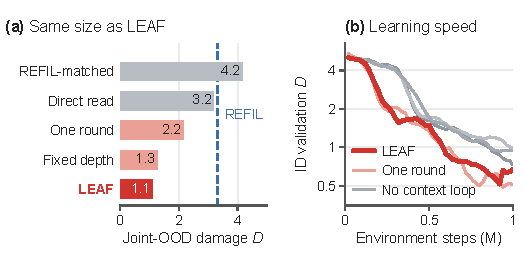
\includegraphics[width=\columnwidth]{figures/exp_capacity.pdf}
\caption{Organization versus size. (a) Joint-OOD damage of the models that share the size of LEAF, 176k parameters. Gray bars mark models that read the entities without a context loop, and red bars models that build the context in a loop. The dashed line marks REFIL, which has 102k parameters. (b) ID validation damage during training, smoothed over five validation points, with REFIL, REFIL-matched, and Direct read drawn in gray. All values are means over three training seeds.}
\label{fig:exp-capacity}
\end{figure}

\begin{figure}[!t]
\centering
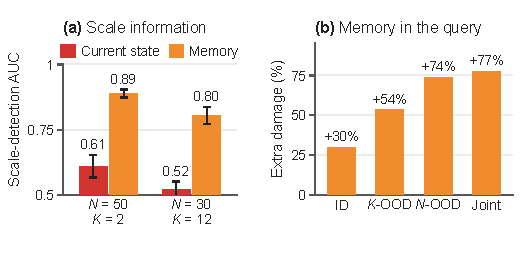
\includegraphics[width=\columnwidth]{figures/exp_memory.pdf}
\caption{Memory after reading. (a) AUC of a linear classifier that separates decisions in a shifted configuration from decisions at $(N,K)=(10,2)$, using either the current self features that form the query of LEAF or its recurrent state $h_{t-1}$. Bars start at the chance level of 0.5, and error bars show one SD over three training seeds. Each configuration contributes ten scenes per model. (b) Extra damage of Memory query, which feeds the recurrent state into the query, relative to LEAF in each group. Joint denotes Joint-OOD.}
\label{fig:exp-memory}
\end{figure}

\begin{figure*}[!t]
\centering
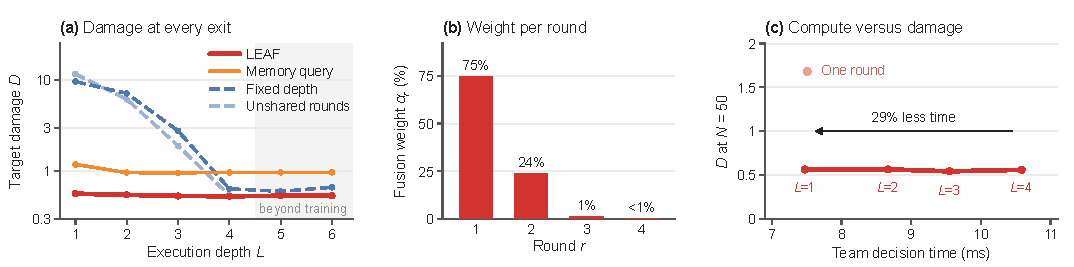
\includegraphics[width=\textwidth]{figures/exp_depth.pdf}
\caption{Execution at any depth. (a) Closed-loop damage at execution depths one to six, averaged over $(N,K)=(10,2)$, $(30,2)$, and $(50,2)$ with 300 scenes each and over three training seeds. Solid lines mark sampled-depth training and dashed lines training at four rounds only. Unshared rounds has no parameters beyond its fourth round, and LEAF comes from a separate depth evaluation with the same protocol. (b) Fusion weight of each round in normal four-round execution of LEAF, averaged over $(10,2)$, $(30,2)$, and $(30,12)$. (c) Full-team decision time and damage at $(50,2)$ for LEAF executed with one to four rounds and for One round. Times come from 20 closed-loop episodes on the workstation described in Section~\ref{subsec:exp-mechanism}, and damage values are means over three training seeds.}
\label{fig:exp-depth}
\end{figure*}

\subsection{Ablation Study}
\label{subsec:exp-ablation}

We next retrain variants of LEAF to identify which designs produce this generalization. All variants share the training budget, seeds, and evaluation of LEAF. Their saved configurations show that consecutive rows of the main chain in Table~\ref{tab:exp-ablation} differ in exactly one switch, so the chain adds the designs of Section~\ref{sec:method} one at a time. Direct read reads the raw entities $H^{(0)}$. One round builds the context for one round before reading, and Fixed depth refines it for four rounds with training at four rounds only. Memory query samples the training depth, and LEAF finally removes the recurrent state from the query. Every variant before LEAF feeds the previous recurrent state into the query with a stopped gradient, so the last step isolates the placement of memory.

Context construction is the foundation. A single context round removes 33\% to 39\% of the damage of Direct read in every group, with the query and training otherwise unchanged. Direct read is exactly the read that Proposition~\ref{prop:selection} restricts, so moving teammates toward or away from a target cannot shift its attention between attackers. After one round, each attacker token already carries information about the target it approaches and the teammates nearby, and the read can weigh attackers by their context.

Refining the context for four rounds lowers damage further, by 33\% in ID and by 51\% and 41\% under team-size and joint extrapolation, and all three seeds improve in both of these groups. In small engagements, one round already captures the relations that matter. With more entities, whether a target is covered depends on relations that a second round composes from the first, as Section~\ref{subsec:method-loop} explains. Multi-round refinement therefore pays off most when the scale grows.

Removing the recurrent state from the query lowers damage by 23\% in ID and by 35\% to 44\% in the extrapolation groups. Seen from LEAF, feeding memory into the query raises damage by 30\% in ID and by 54\% to 77\% under extrapolation, and the spread across seeds grows with it. Under joint extrapolation, the SD rises from 0.10 for LEAF to 1.23 for Memory query. Memory placement thus matters most where deployment departs furthest from training, and Section~\ref{subsec:exp-mechanism} traces this effect to drift of the recurrent state.

Sampling the training depth raises the four-round damage within the memory-query family, mostly through one of the three training runs. LEAF also samples its depth and matches or improves on Fixed depth in all four groups. The value of sampled depth lies in the shallower exits, which Section~\ref{subsec:exp-mechanism} examines. Untying the rounds in Unshared rounds or reading only the last round in Last read leaves the four-round damage close to that of LEAF, and these choices matter when the execution depth changes. Removing the REFIL host in No host raises damage in all three extrapolation groups, so LEAF builds on the entity grouping of its host.

\subsection{Mechanism Analysis}
\label{subsec:exp-mechanism}

Finally, we examine why LEAF works through three properties of its computation. The gain comes from how the computation is organized, reading the scene from the current state keeps its interpretation stable as memory drifts, and sampled-depth training makes every execution depth a usable policy.

\emph{Organization over size.} REFIL-matched widens the actor of REFIL with a residual multilayer perceptron to within 0.4\% of the parameter count of LEAF. Its damage is 2.3 to 3.9 times that of LEAF and higher than that of REFIL in all four groups. Fig.~\ref{fig:exp-capacity}(a) compares the models that share the size of LEAF. Their joint-extrapolation damage spans almost a factor of four, and every model that builds the context in a loop incurs less damage than REFIL. Size does not predict damage across methods either. ALMA has as many parameters as Unshared rounds and more than four times its joint-extrapolation damage. Context construction also speeds up learning. In Fig.~\ref{fig:exp-capacity}(b), One round learns at the pace of LEAF, whereas Direct read and REFIL-matched follow REFIL. The trained policy relies on this context. When the frozen LEAF policy reads the raw entities $H^{(0)}$ in place of its context, damage rises in all nine combinations of model and configuration that we tested, with ten scenes each.

\emph{Memory after reading.} Section~\ref{subsec:method-memory} argued that a recurrent state accumulated in a larger engagement can leave the range seen in training. We test this with a probe~\cite{alain2017probes}. For each training seed, a classifier separates decisions in a shifted configuration from decisions at $(N,K)=(10,2)$, using either the recurrent state $h_{t-1}$ of LEAF or the current self features from which its query is formed. In Fig.~\ref{fig:exp-memory}(a), a linear classifier identifies the deployment scale from the recurrent state with an area under the receiver operating characteristic curve (AUC) of 0.89 at $(50,2)$ and 0.80 at $(30,12)$. From the current self features it reaches only 0.61 and 0.52. Gradient-boosted trees give the same picture, and every seed agrees. Memory learned in small engagements thus moves into new regions as the scale grows, while the current self state stays close to the training distribution. The query is a deterministic function of the self features, so it carries no more scale information than they do.

Feeding memory into the query carries this drift into the reading of the scene. Fig.~\ref{fig:exp-memory}(b) shows that the extra damage of Memory query grows from 30\% in ID to 77\% under joint extrapolation, and Table~\ref{tab:exp-ablation} shows that its seeds spread further apart. Team behavior follows the same order. In the four configurations with protection records, Memory query lies between REFIL and LEAF on interception, damage incidence, tail damage, and friendly collisions in all 16 comparisons. Memory remains useful downstream. Resetting the recurrent state of the frozen LEAF policy at every step raises damage in eight of nine combinations of model and configuration. LEAF therefore keeps memory for selecting intents and keeps it out of the step that reads the threat context.

\emph{Every exit is a usable policy.} In normal four-round execution, the first two rounds receive about 99\% of the fusion weight in every configuration we examined, and the first round alone about three quarters, as Fig.~\ref{fig:exp-depth}(b) shows. The split varies across defenders, with an SD of 11 to 14 percentage points among the defenders of the same state, so each defender draws on the rounds in its own way. Proposition~\ref{prop:prefix} links this small fusion mass beyond the second round to stable decisions. We execute two rounds instead of four in the same states for 48{,}705 decisions at $(10,2)$, $(50,2)$, and $(30,12)$, with ten scenes per model. The greedy intent changes in only 1.1\% to 1.7\% of the decisions. For 79\% of them, the utility gap exceeds twice the largest utility change $\delta$ between the two depths, the condition of the proposition, so these decisions keep their intent. The decisions that do change lie mostly in the lowest tenth of utility gaps, 78\% to 81\% of them, where the two best intents are nearly equivalent.

Closed-loop execution confirms the same picture. Over all 24 configurations, executing two rounds instead of four changes the damage of LEAF by about 1\%, and a single round by about 2\%. Executing five or six rounds, beyond the training range, changes it by less than 0.1\%. Sampled-depth training is what keeps the shallow exits usable. Memory query and Fixed depth share the architecture and the query and differ only in how the training depth is chosen. In Fig.~\ref{fig:exp-depth}(a), the two sampled-depth models stay flat from one to six rounds. Fixed depth executed for one round incurs 15 times its own four-round damage. Five of the six models trained at four rounds collapse in this way, whereas all six sampled-depth models stay within a factor of 1.5 of their four-round damage.

A shorter exit saves computation at deployment. We time the policies on a workstation with an NVIDIA GeForce RTX 5070 Ti GPU and an Intel Core i7-14700KF CPU, using PyTorch 2.13 with CUDA 13.0. A full-team decision for 50 defenders takes 7.5~ms with one round and 10.6~ms with four, two orders of magnitude below the decision interval of 1~s. An operator can therefore cut the decision time by 29\% without retraining, at a cost of about 2\% in average damage. Fig.~\ref{fig:exp-depth}(c) adds that LEAF executed for one round runs as fast as One round, the model trained with a single round, and incurs about one third of its damage at $(50,2)$.
